\section{Data Gathering and Visualization Approaches}\label{sec:methods}
In the pursuit of optimizing a program's data locality, implementing visual aids to represent data movements and data layouts can be particularly helpful. This approach enables quick and effective identification of data-related issues, their comprehension, and ultimately, their resolution. This method empowers not only program optimization experts but also domain researchers to effortlessly optimize their programs.

To enable such effective visualization, however, it's essential to first collect information regarding data locality. Several studies have explored this area, leading to the identification of three primary strategies: Dynamic Analysis, Static Analysis, and Simulation. These strategies, which we'll delve into in Sections \ref{sec:dynamic_analysis}, \ref{sec:static_analysis}, and \ref{sec:simulation}, each bring their unique benefits and drawbacks. Furthermore, it's important to note that some techniques used for gathering data locality information may not be confined to just one of these three fundamental categories, and could instead exhibit characteristics of multiple approaches.

Once this data locality information is gathered, it needs to be presented in a user-friendly manner. There exists a wide variety of visualization techniques that can fulfill this requirement, some of which we will detail in Section \ref{sec:visualization}.

\subsection{Dynamic Analysis}\label{sec:dynamic_analysis}
Dynamic analysis of a program's data locality involves executing the program while concurrently gathering memory-related data and statistics. A straightforward approach to dynamic analysis is to run the program, extract hardware counters such as cache misses, and analyze them. This approach, however, does not provide a holistic view of the program's behavior because it lacks contextual information.

To gain a deeper understanding of program performance beyond general statistics, dynamic analysis uses more nuanced techniques like profiling, statistical sampling, and tracing \cite{shende1999profiling,itzkowitz2003memory,gimenez2017memaxes,mckinley1999quantifying,adhianto2010hpctoolkit}.

Profiling involves periodically interrupting the program's execution to capture both hardware-derived attributes and context-related information \cite{itzkowitz2003memory,gimenez2017memaxes,adhianto2010hpctoolkit}. Profiling techniques analyze the program's call stack and program counter to provide specific details such as the current line of code being executed, the symbol, and, for arrays, the accessed index. This information facilitates the derivation of deeper metrics, such as the number of cache misses per array \cite{adhianto2010hpctoolkit}. Profiling typically focuses on memory-related events, but the constant interruption can increase runtime overhead. Hence, a trade-off between the granularity and the quality of the measurements is necessary.

Statistical sampling is an alternative approach related to profiling. It captures the program's state at fixed time intervals rather than event-triggered interruptions. The advantage of statistical sampling is that it avoids frequent interruption of the program's execution, reducing the runtime overhead. However, high-quality measurements require sufficiently high sampling rates to capture all relevant details \cite{adhianto2010hpctoolkit}.

Tracing, another technique, allows for a temporal understanding of a program's behavior by logging event-specific data over time. Tracing functions by documenting specific events or functions during program execution, providing a chronological account of these events and their corresponding data \cite{shende1999profiling,adhianto2010hpctoolkit,mckinley1999quantifying}.

In conclusion, dynamic analysis offers several distinct advantages in the study of a program's behavior concerning data locality. As the program is being executed, it offers more precise practical insights into hardware oriented data locality optimization. Further, dynamic analysis can be employed in conjunction with actual data, making it more representative of real-world scenarios.

However, it's important to note the inherent disadvantages of dynamic analysis. The act of running an entire program can be time-consuming and costly, particularly for larger and more complex software. Additionally, isolating and scrutinizing specific parts of a program under the dynamic analysis approach can be complicated, especially when compared to static analysis methods (Section \ref{sec:static_analysis}).

\subsection{Static Analysis}\label{sec:static_analysis}
\begin{figure}
  \centering
  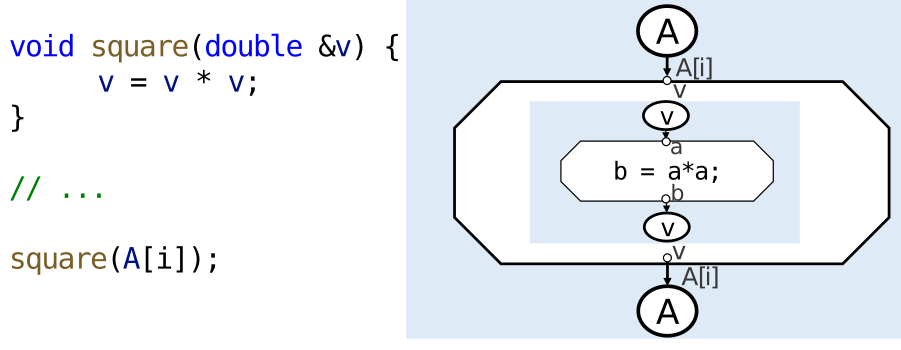
\includegraphics[width=\linewidth]{pictures/SDFG.png}
  \caption{\texttt{C} language source code and its corresponding SDFG representation \cite{calotoiu2022lifting}.}
  \label{fig:sdfg}
\end{figure}

\begin{figure*}
	\begin{subfigure}[c]{.30\textwidth}
		\centering
		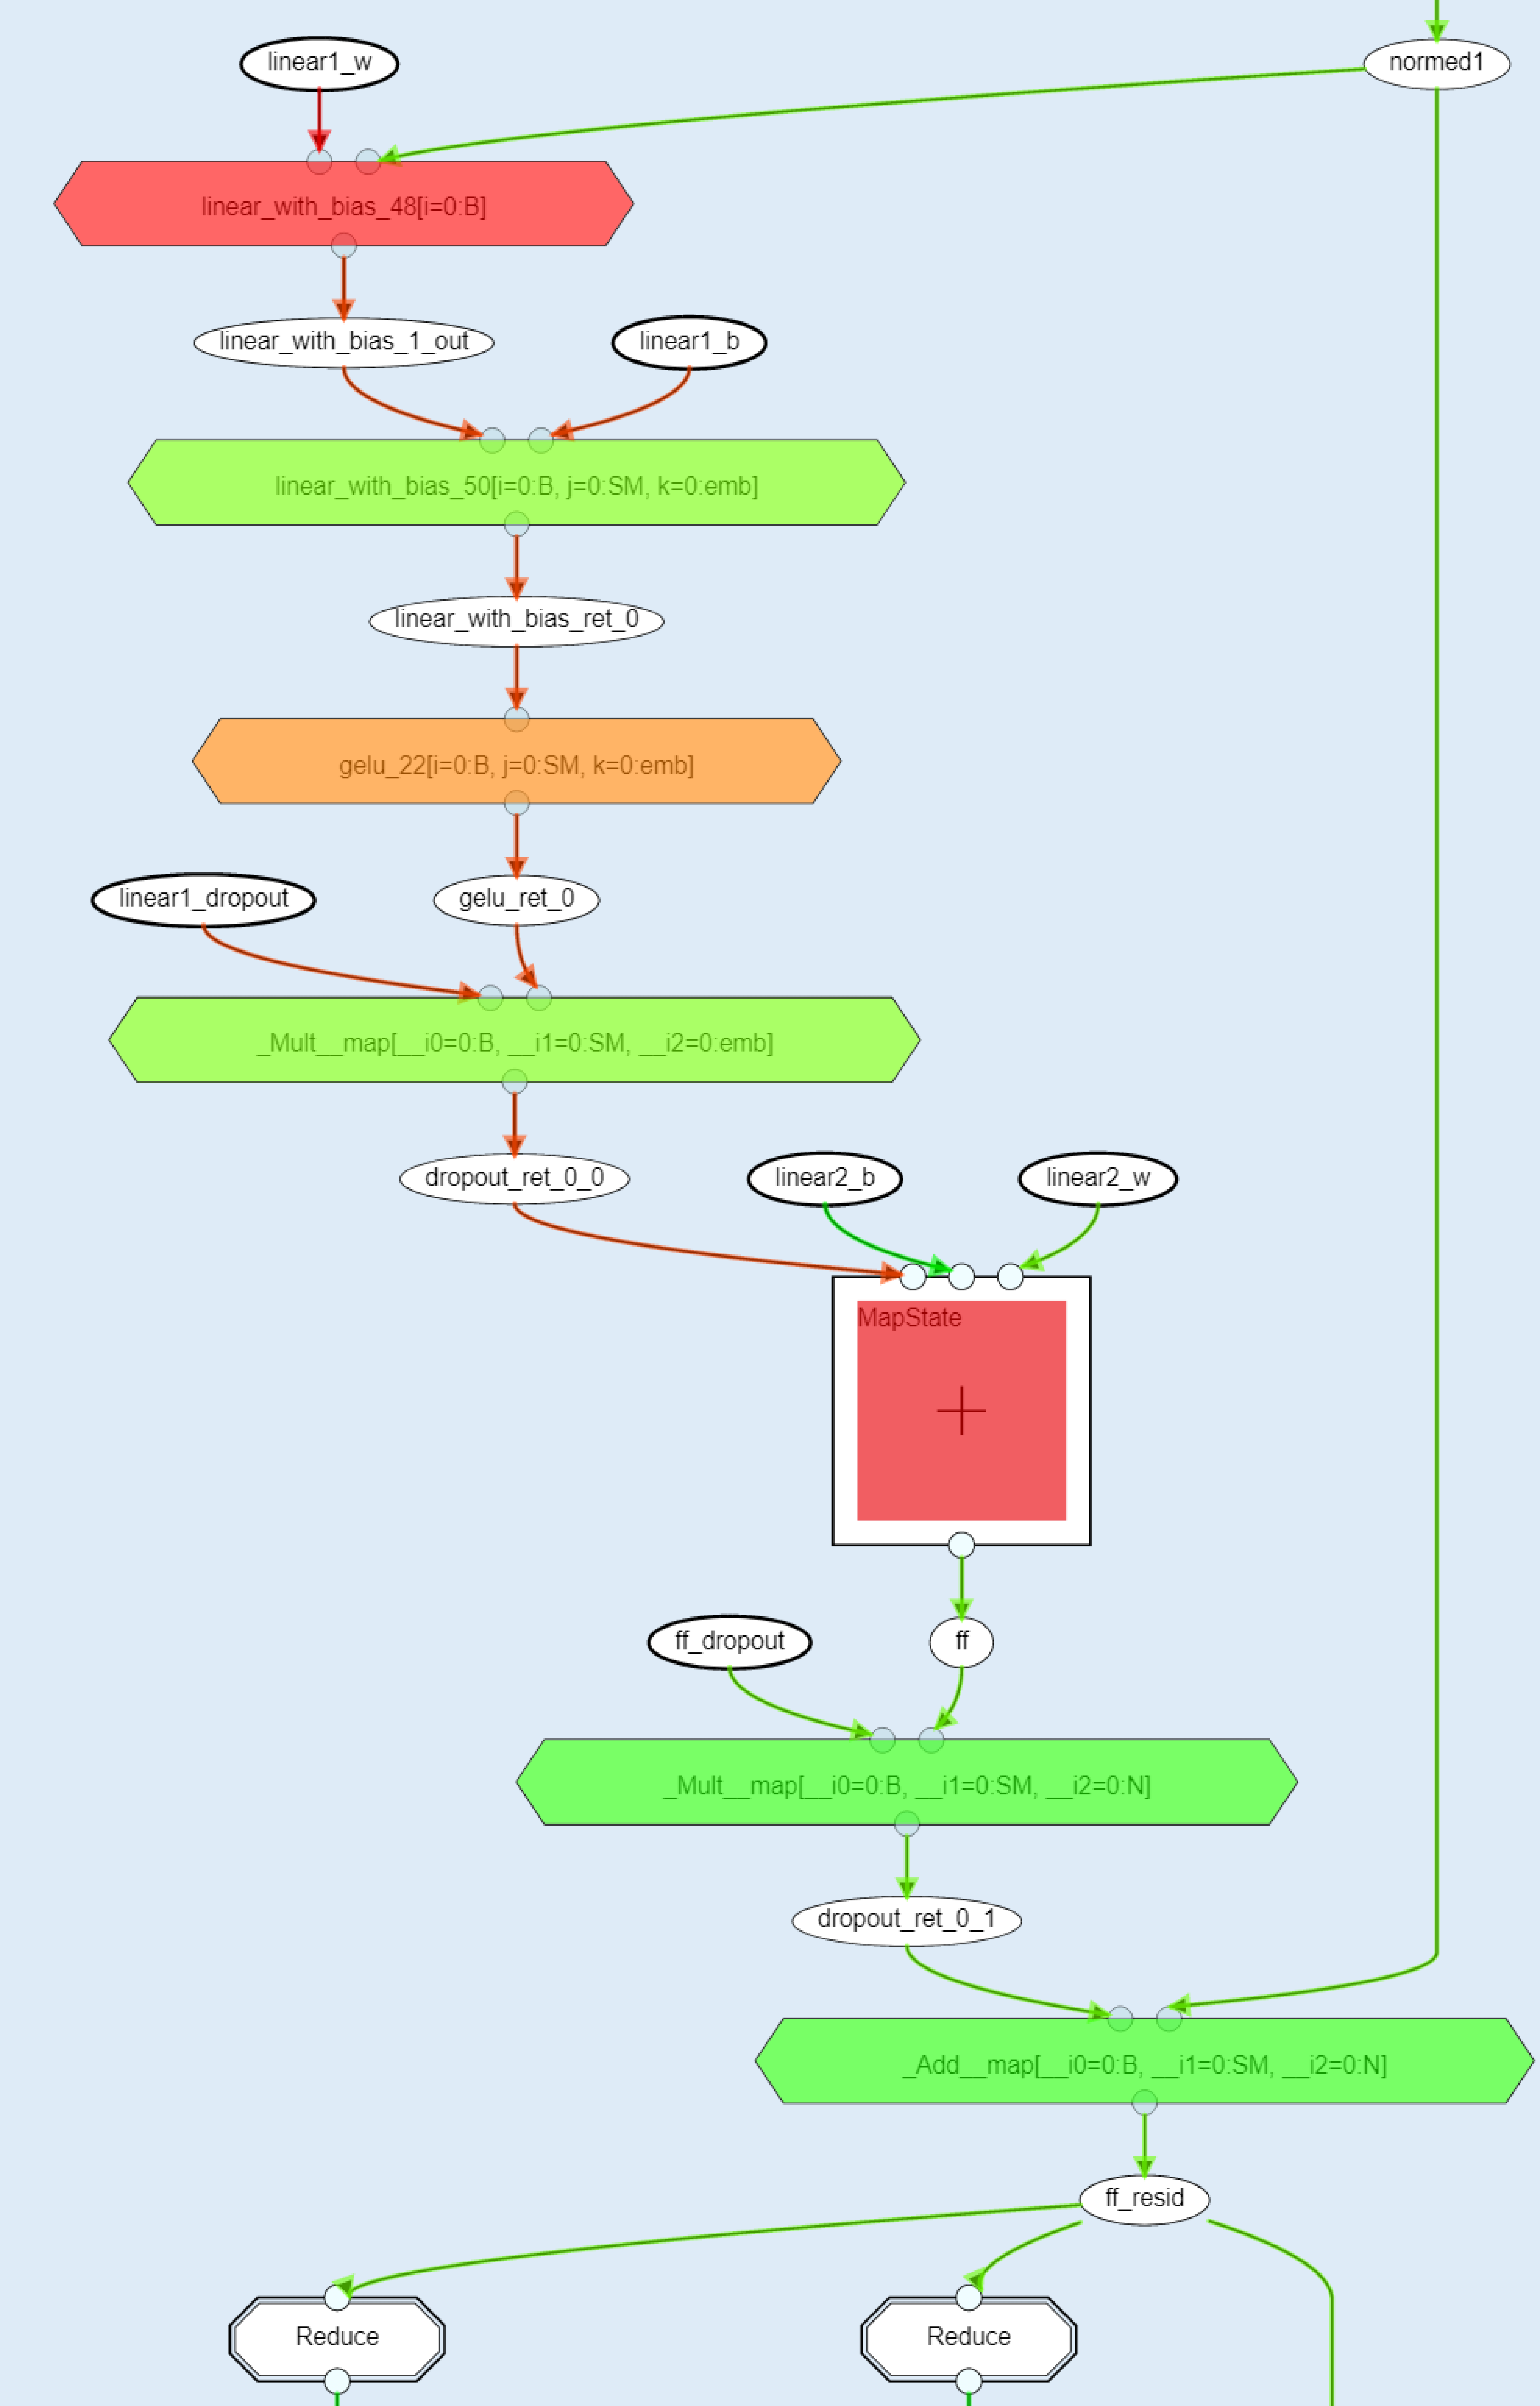
\includegraphics[width=\linewidth]{pictures/boosting_master_both.png}
	\end{subfigure}
	\begin{subfigure}[c]{.68\textwidth}
		\centering
		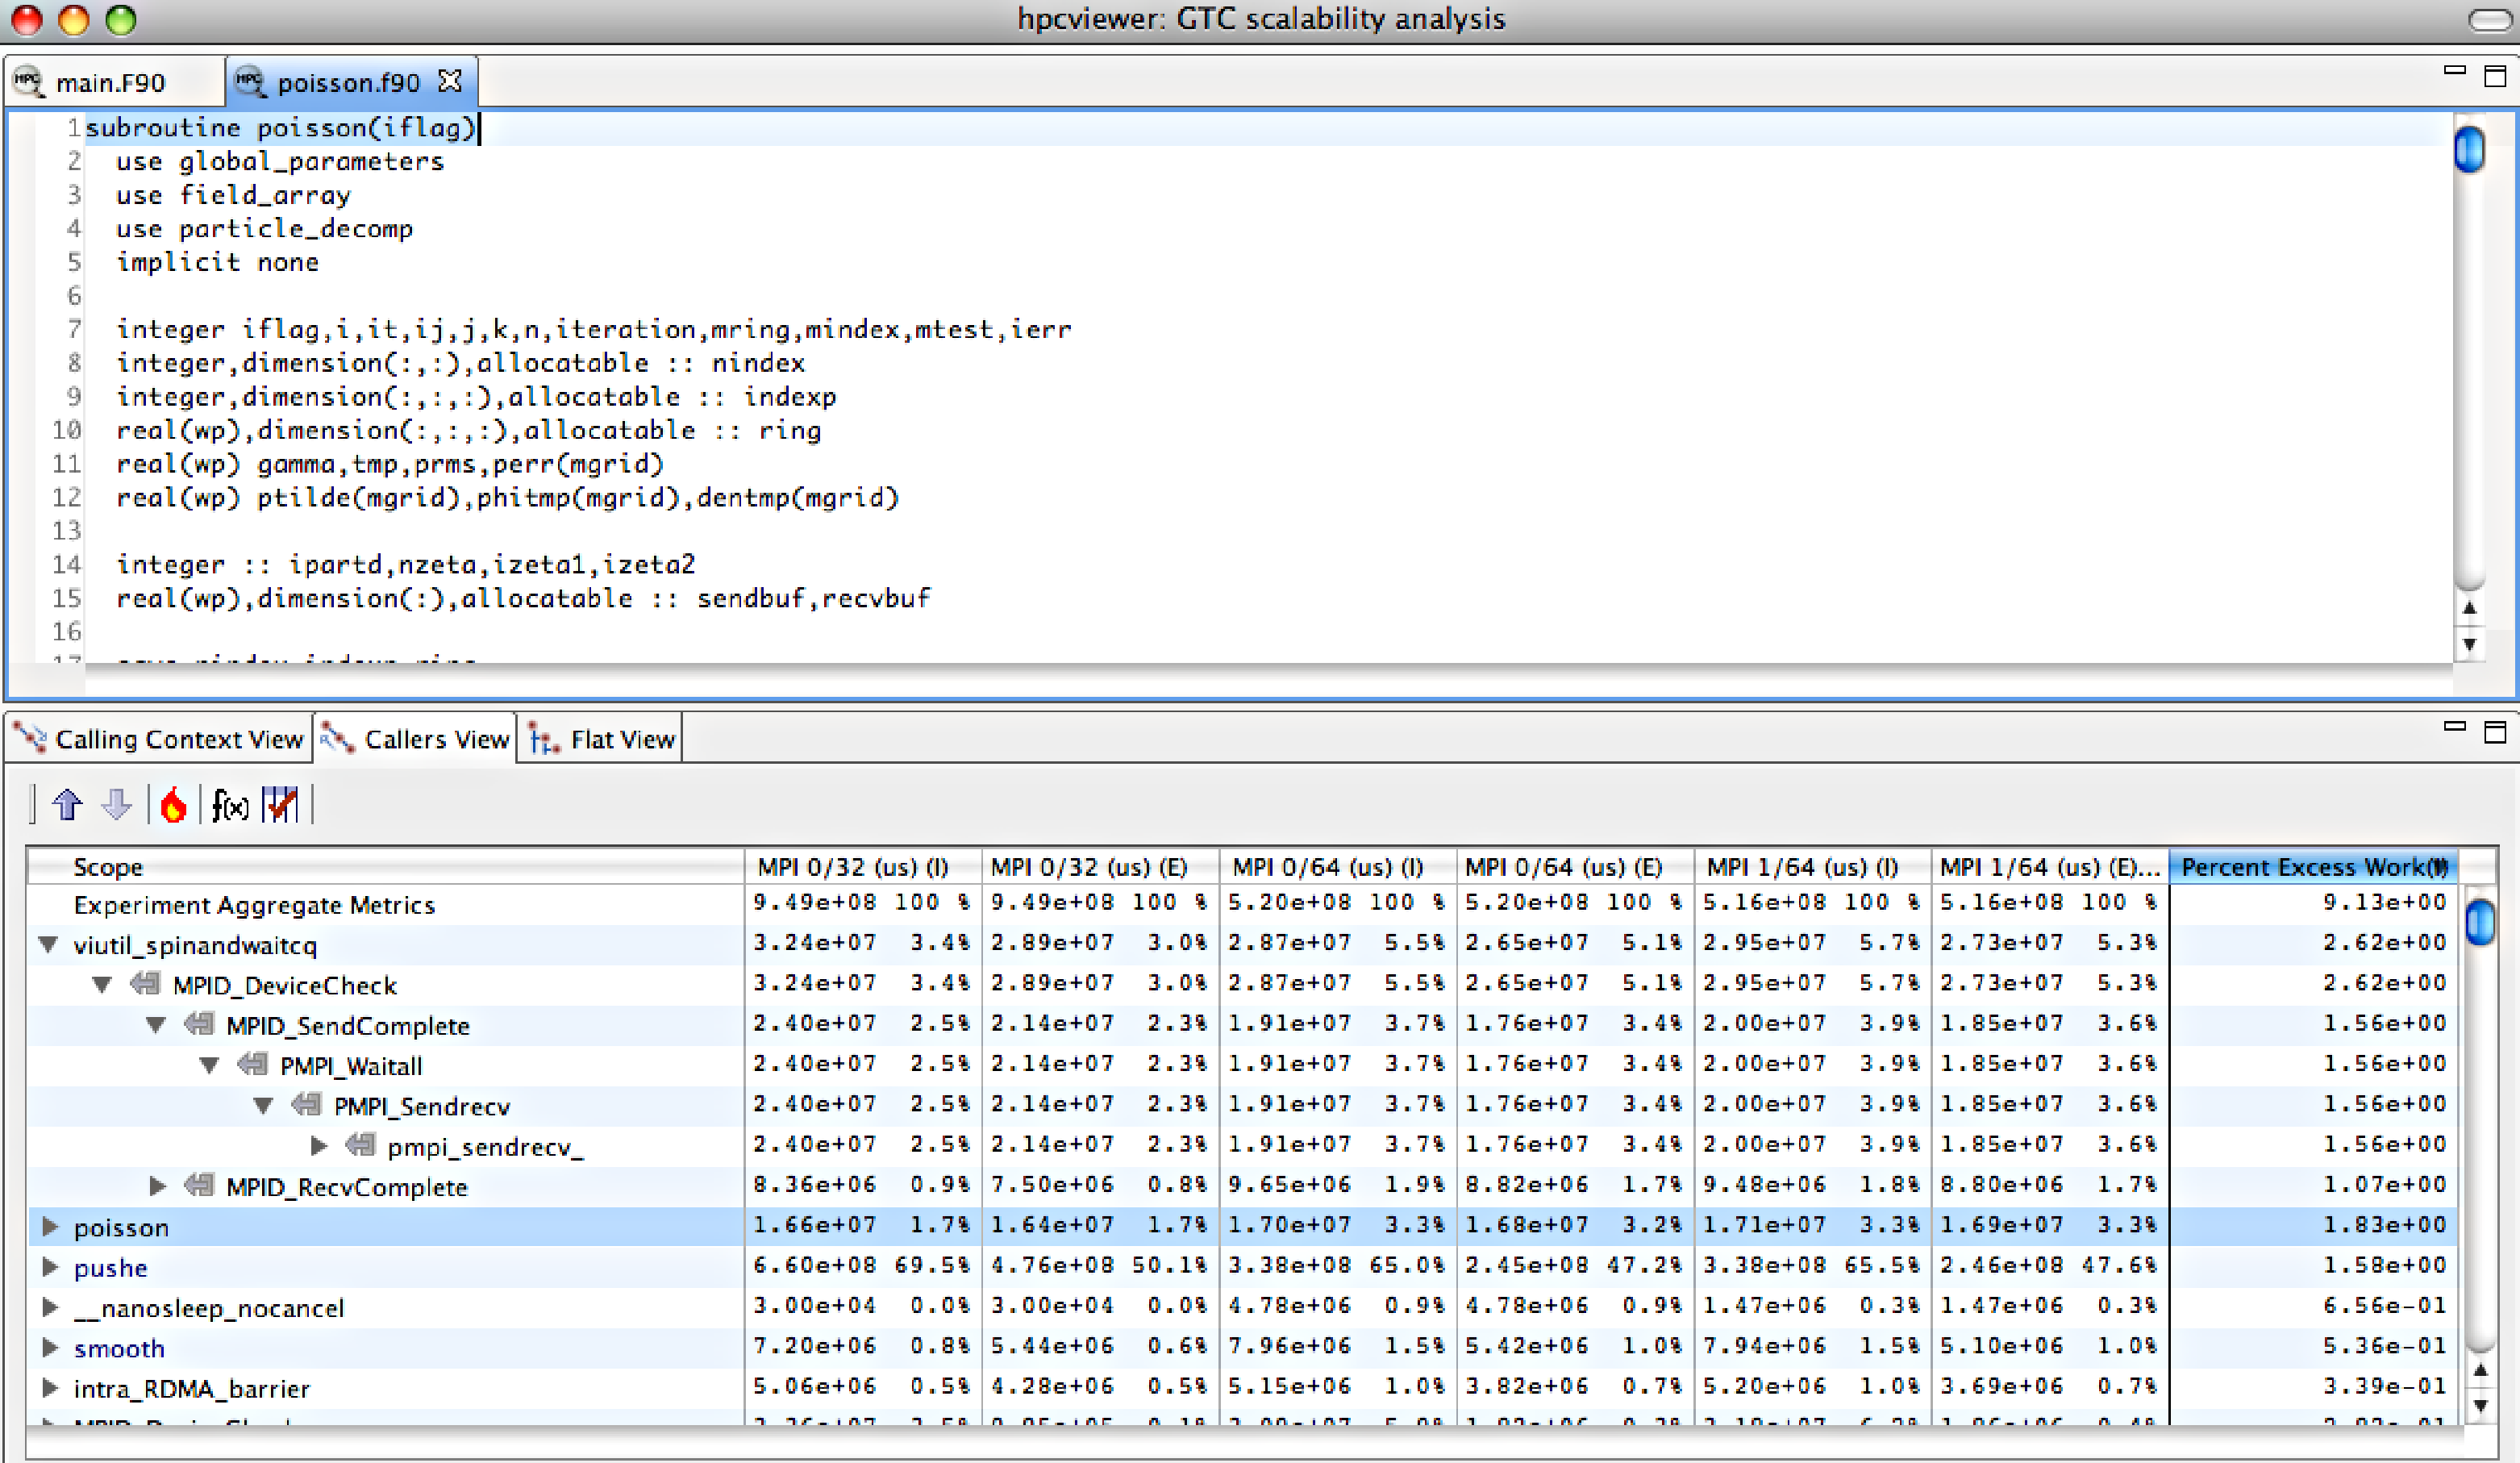
\includegraphics[width=\linewidth]{pictures/hpctoolkitviewer.png}
	\end{subfigure}
	\caption{Left: Coloring in memory volume onto memlets and arithmetic intensity onto tasklets in an SDFG \cite{schaad2021boosting}. Right: \texttt{HPCToolkit}'s viewer, which displays the program's source code and its corresponding memory access information \cite{adhianto2010hpctoolkit}.}
	\label{fig:coarse}
\end{figure*}

Unlike dynamic analysis, static analysis takes a different tack in examining a program's data locality. Instead of operating the program in real-time to gather data, static analysis scrutinizes the program's source code itself. By transforming the source code into an intermediate representation (IR) that centers on data, and subsequently analyzing this IR, static analysis is able to uncover memory-related issues \cite{schaad2022boosting,schaad2021boosting,calotoiu2022lifting,ben2023bridging}.

There are myriad IRs in use, like MLIR, which are predominantly control-flow oriented, facilitating optimizations pivoting around control elements like loop restructuring \cite{moses2021polygeist}. However, in the context of data locality, data-centric IRs such as SDFG (\cite{ben2019statefulSDFG}), PROGRAPH (\cite{matwin1985prograph}), and LabVIEW (\cite{kodosky2020labview}) provide a more direct approach. By prioritizing memory, its movements, and its computation-induced alterations, these IRs allow for both automated (\cite{ben2019statefulSDFG}) and, when paired with visual aids, manual enhancements of data locality \cite{ben2023bridging,ben2019statefulSDFG,schaad2021boosting}.

Taking the example of SDFGs, the entire data flow of a program can be represented as a directed graph. Nodes within this graph symbolize $N$-dimensional arrays of data, computations (tasklets), or map scopes that denote general parallelism (such as loops). The edges, or memlets, in an SDFG represent explicit data movements \cite{ben2019statefulSDFG}. An example of the SDFG IR is provided in Figure \ref{fig:sdfg}.

As the SDFG IR of a program is constructed, it is possible to compute memory-related properties crucial for data locality. For instance, each memlet carries information regarding the volume of data transported between nodes \cite{ben2019statefulSDFG}, and tasklets and nested SDFGs can be annotated with metadata related to the number of executions and arithmetic operations undertaken \cite{schaad2021boosting}. Consequently, SDFGs offer a comprehensive view of the program and facilitate the identification of data movement bottlenecks on a large scale.

Despite static analysis's robust capability for macroscopic program analysis - a trait not shared with dynamic analysis - it does not provide the same level of detail. Given that performance bottlenecks are often induced by memory accesses that are tied to physical access patterns and hence are hardware-specific, static analysis alone may not accurately predict, say, the number of cache misses for a particular function. However, the advantage of static analysis lies in the fact that it does not necessitate program execution, thereby enabling quicker and cost-effective optimization of logical data movements compared to dynamic analysis.

\subsection{Cache Simulation}\label{sec:simulation}

Positioned between dynamic and static analysis lies the realm of simulation-based approaches, of which cache simulation is particularly noteworthy. Cache simulation is a method used to simulate a program's data accesses on a virtual memory hierarchy model. This process allows for an in-depth examination of both spatial and temporal data locality, as elaborated on in Section \ref{sec:data_locality}.

The process of setting up a cache simulator can be divided into two ways:

In the first approach, the program is pseudo-executed without implementing any real computations. This process starts by constructing a virtual memory hierarchy that includes caches. As the program proceeds through its lifecycle:
\begin{itemize}
	\item Corresponding space is allocated in the simulated memory for each instance of allocation, and reciprocally, space is deallocated as per the program's instructions.
	\item The simulator emulates each memory access operation, both read and write, according to how a CPU would handle the task. This entails an initial probe in the L1 cache, followed by a potential cache miss procedure if the required data is absent, as discussed in Section \ref{sec:data_transfer}.
\end{itemize}
This methodology facilitates a comprehensive and accurate representation of the system's memory hierarchy and its interaction with the computing process \cite{schaad2022boosting,hammer2017kerncraft}.

The second approach uses dynamic analysis (Section \ref{sec:dynamic_analysis}) to generate memory traces. These traces are then rerun through the simulator, enabling an enriched understanding of memory access and management behavior within the program \cite{choudhury2011abstract}.

The deployment of cache simulators extends beyond mere prediction of cache misses. When operated in a step-by-step manner, these tools permit the exploration of data access patterns of a procedure at a granular level. Such detailed inspection can uncover potential enhancements in spatial locality, either through modifications in data layout or access strategies, ultimately contributing to improved performance \cite{schaad2022boosting,hammer2017kerncraft,choudhury2011abstract}.

Moreover, cache simulation enables close-up performance analysis of a program, such as focusing on a single function within the source code or limiting memory traces to a specific functional context.

Despite its advantages, cache simulation demands an in-depth understanding of the target architecture, including aspects like cache hierarchy, cache replacement policy, and cache coherence protocol. Any inaccuracies in these parameters can lead to misleading results, potentially causing optimization attempts to inadvertently degrade the program's data locality.

\subsection{Visualization Techniques}\label{sec:visualization}
\begin{figure}
	\centering
	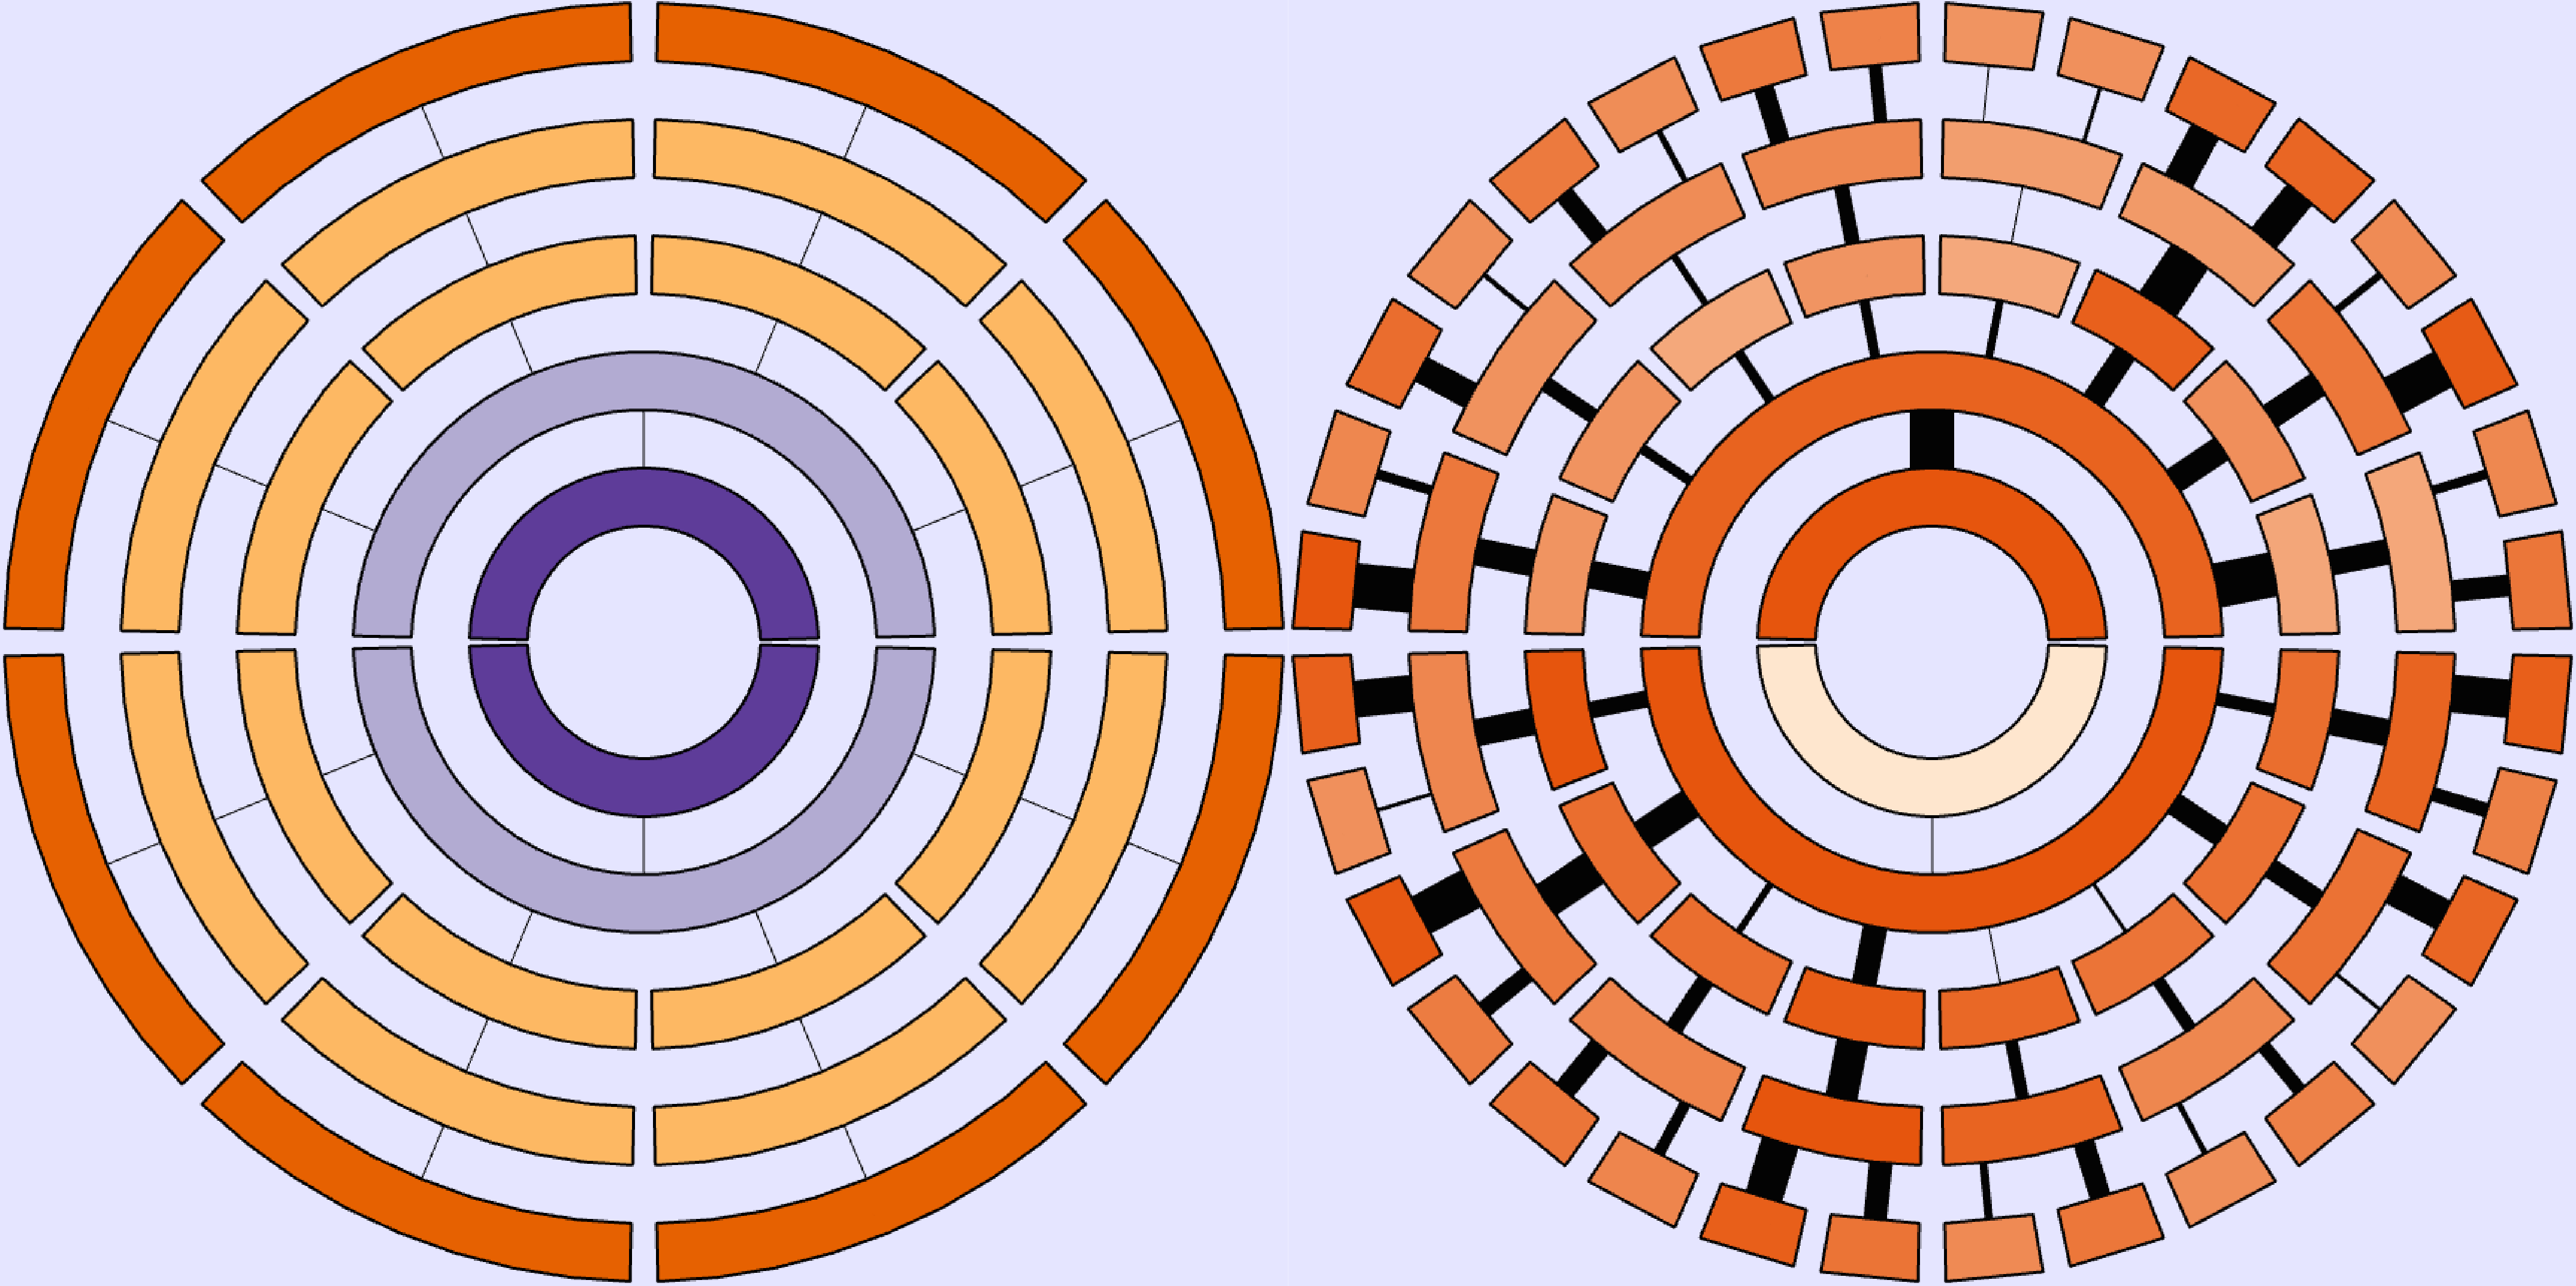
\includegraphics[width=\linewidth]{pictures/memaxes_cache.png}
	\caption{Left: A radial design representing the hardware topology. Main memory resources are depicted in deep purple and processing units in dark orange, with different layers of caches in between. Right: An complex architecture is portrayed, featuring performance data tagged onto the hardware resources through a color code, and transactions among them indicated by line thickness \cite{gimenez2017memaxes}.}
	\label{fig:memaxes_cache}
\end{figure}
\begin{figure}
	\centering
	\begin{subfigure}[c]{.54\linewidth}
		\centering
		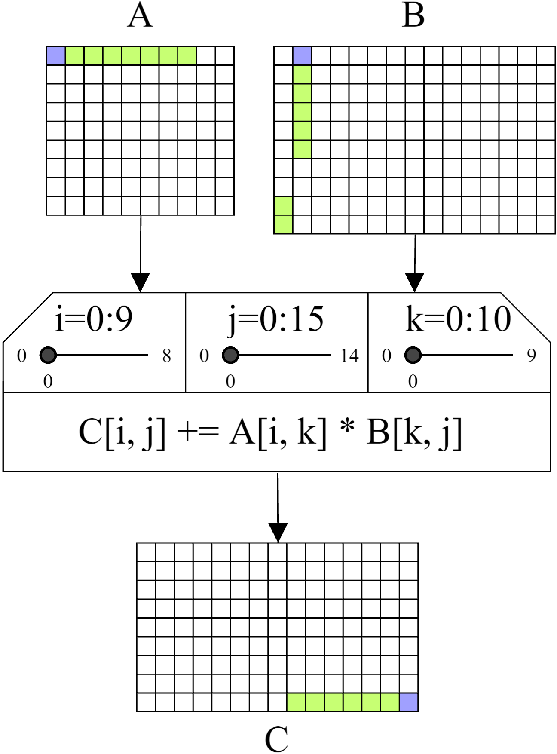
\includegraphics[width=\linewidth]{pictures/boosting_cache_lines.png}
	\end{subfigure}
	\begin{subfigure}[c]{.44\linewidth}
		\centering
		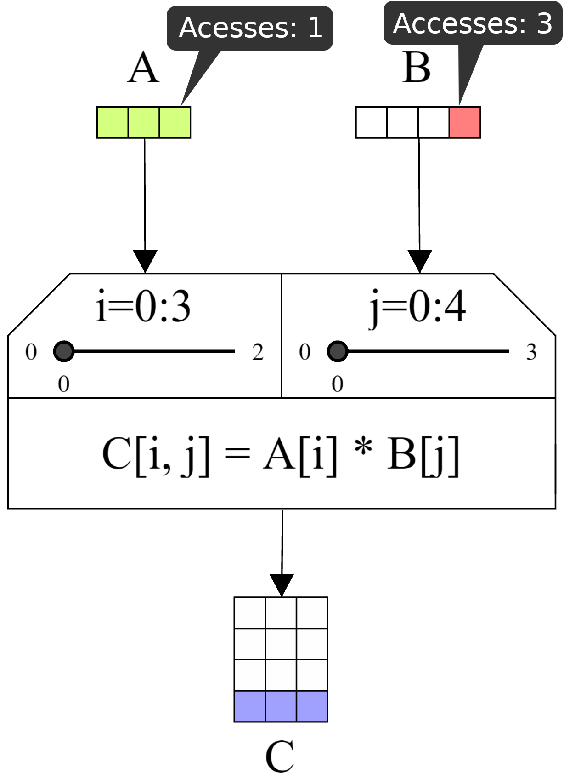
\includegraphics[width=\linewidth]{pictures/boosting_access_patterns.png}
	\end{subfigure}
	\caption{Left: Illustration of data layouts emphasizing spatial locality via cache lines. Right: Visualization of correlated accesses to elements $A$ and $B$ with respect to accesses to $C[3,x], x \in \{0,1,2\}$ \cite{schaad2022boosting}.}
	\label{fig:boosting_cache}
\end{figure}

\begin{figure*}
	\begin{subfigure}[c]{.48\linewidth}
		\centering
		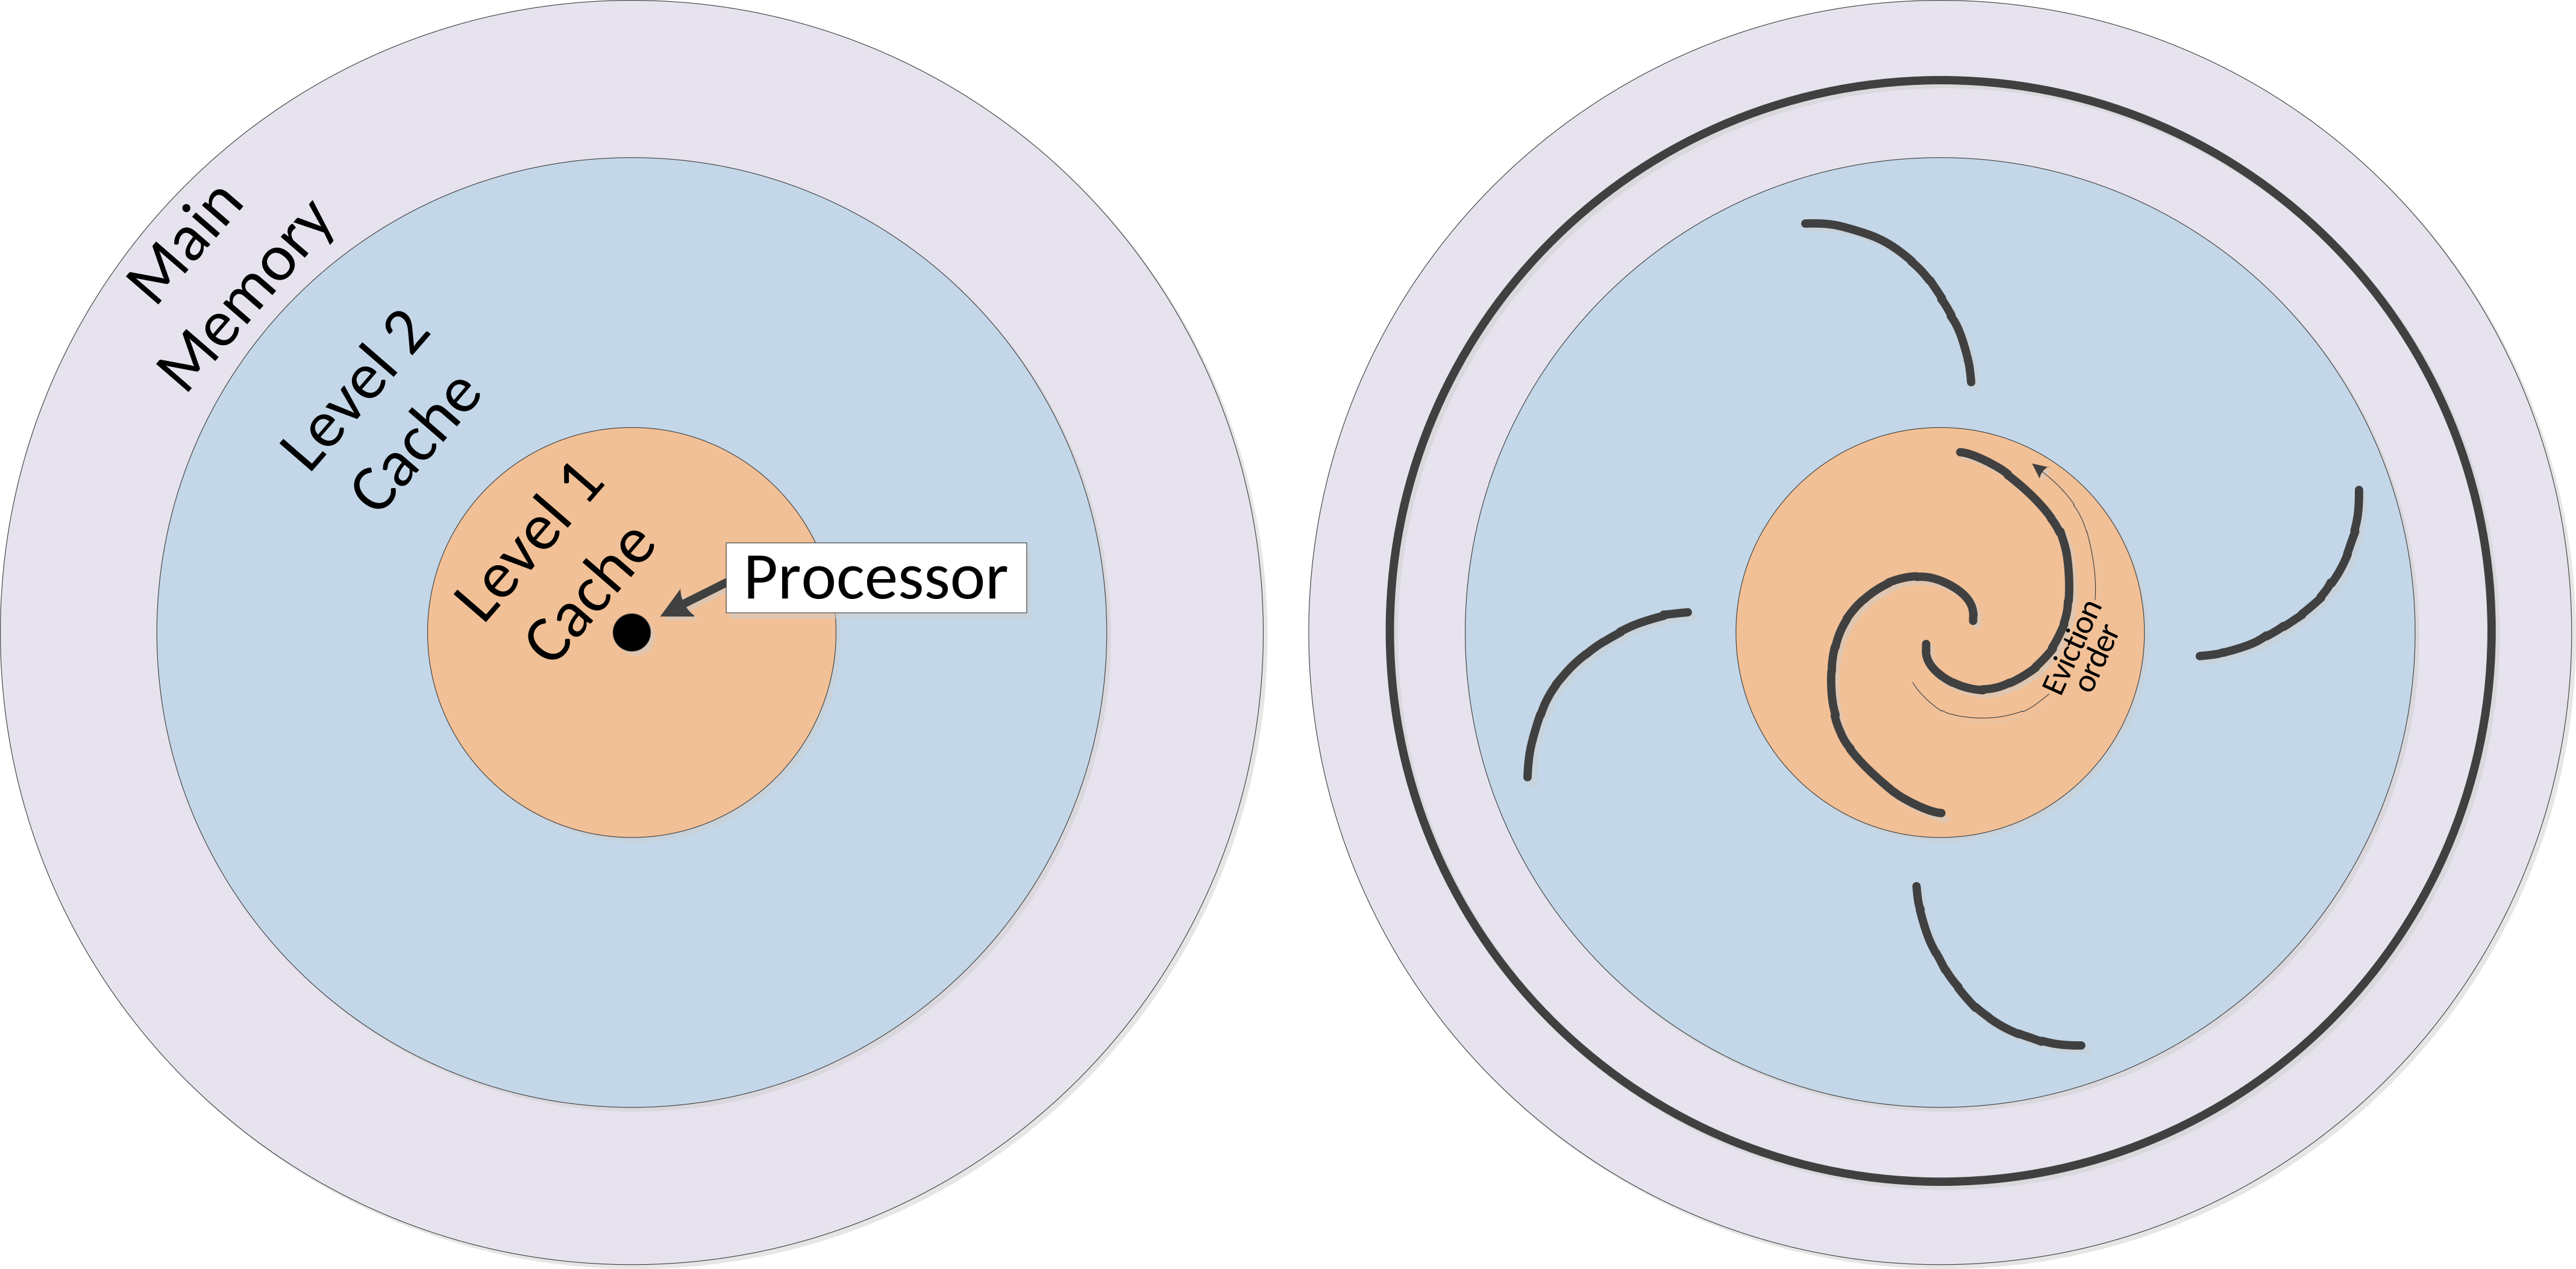
\includegraphics[width=\linewidth]{pictures/abstract_explanation.png}
	\end{subfigure}
	\begin{subfigure}[c]{.24\linewidth}
		\centering
		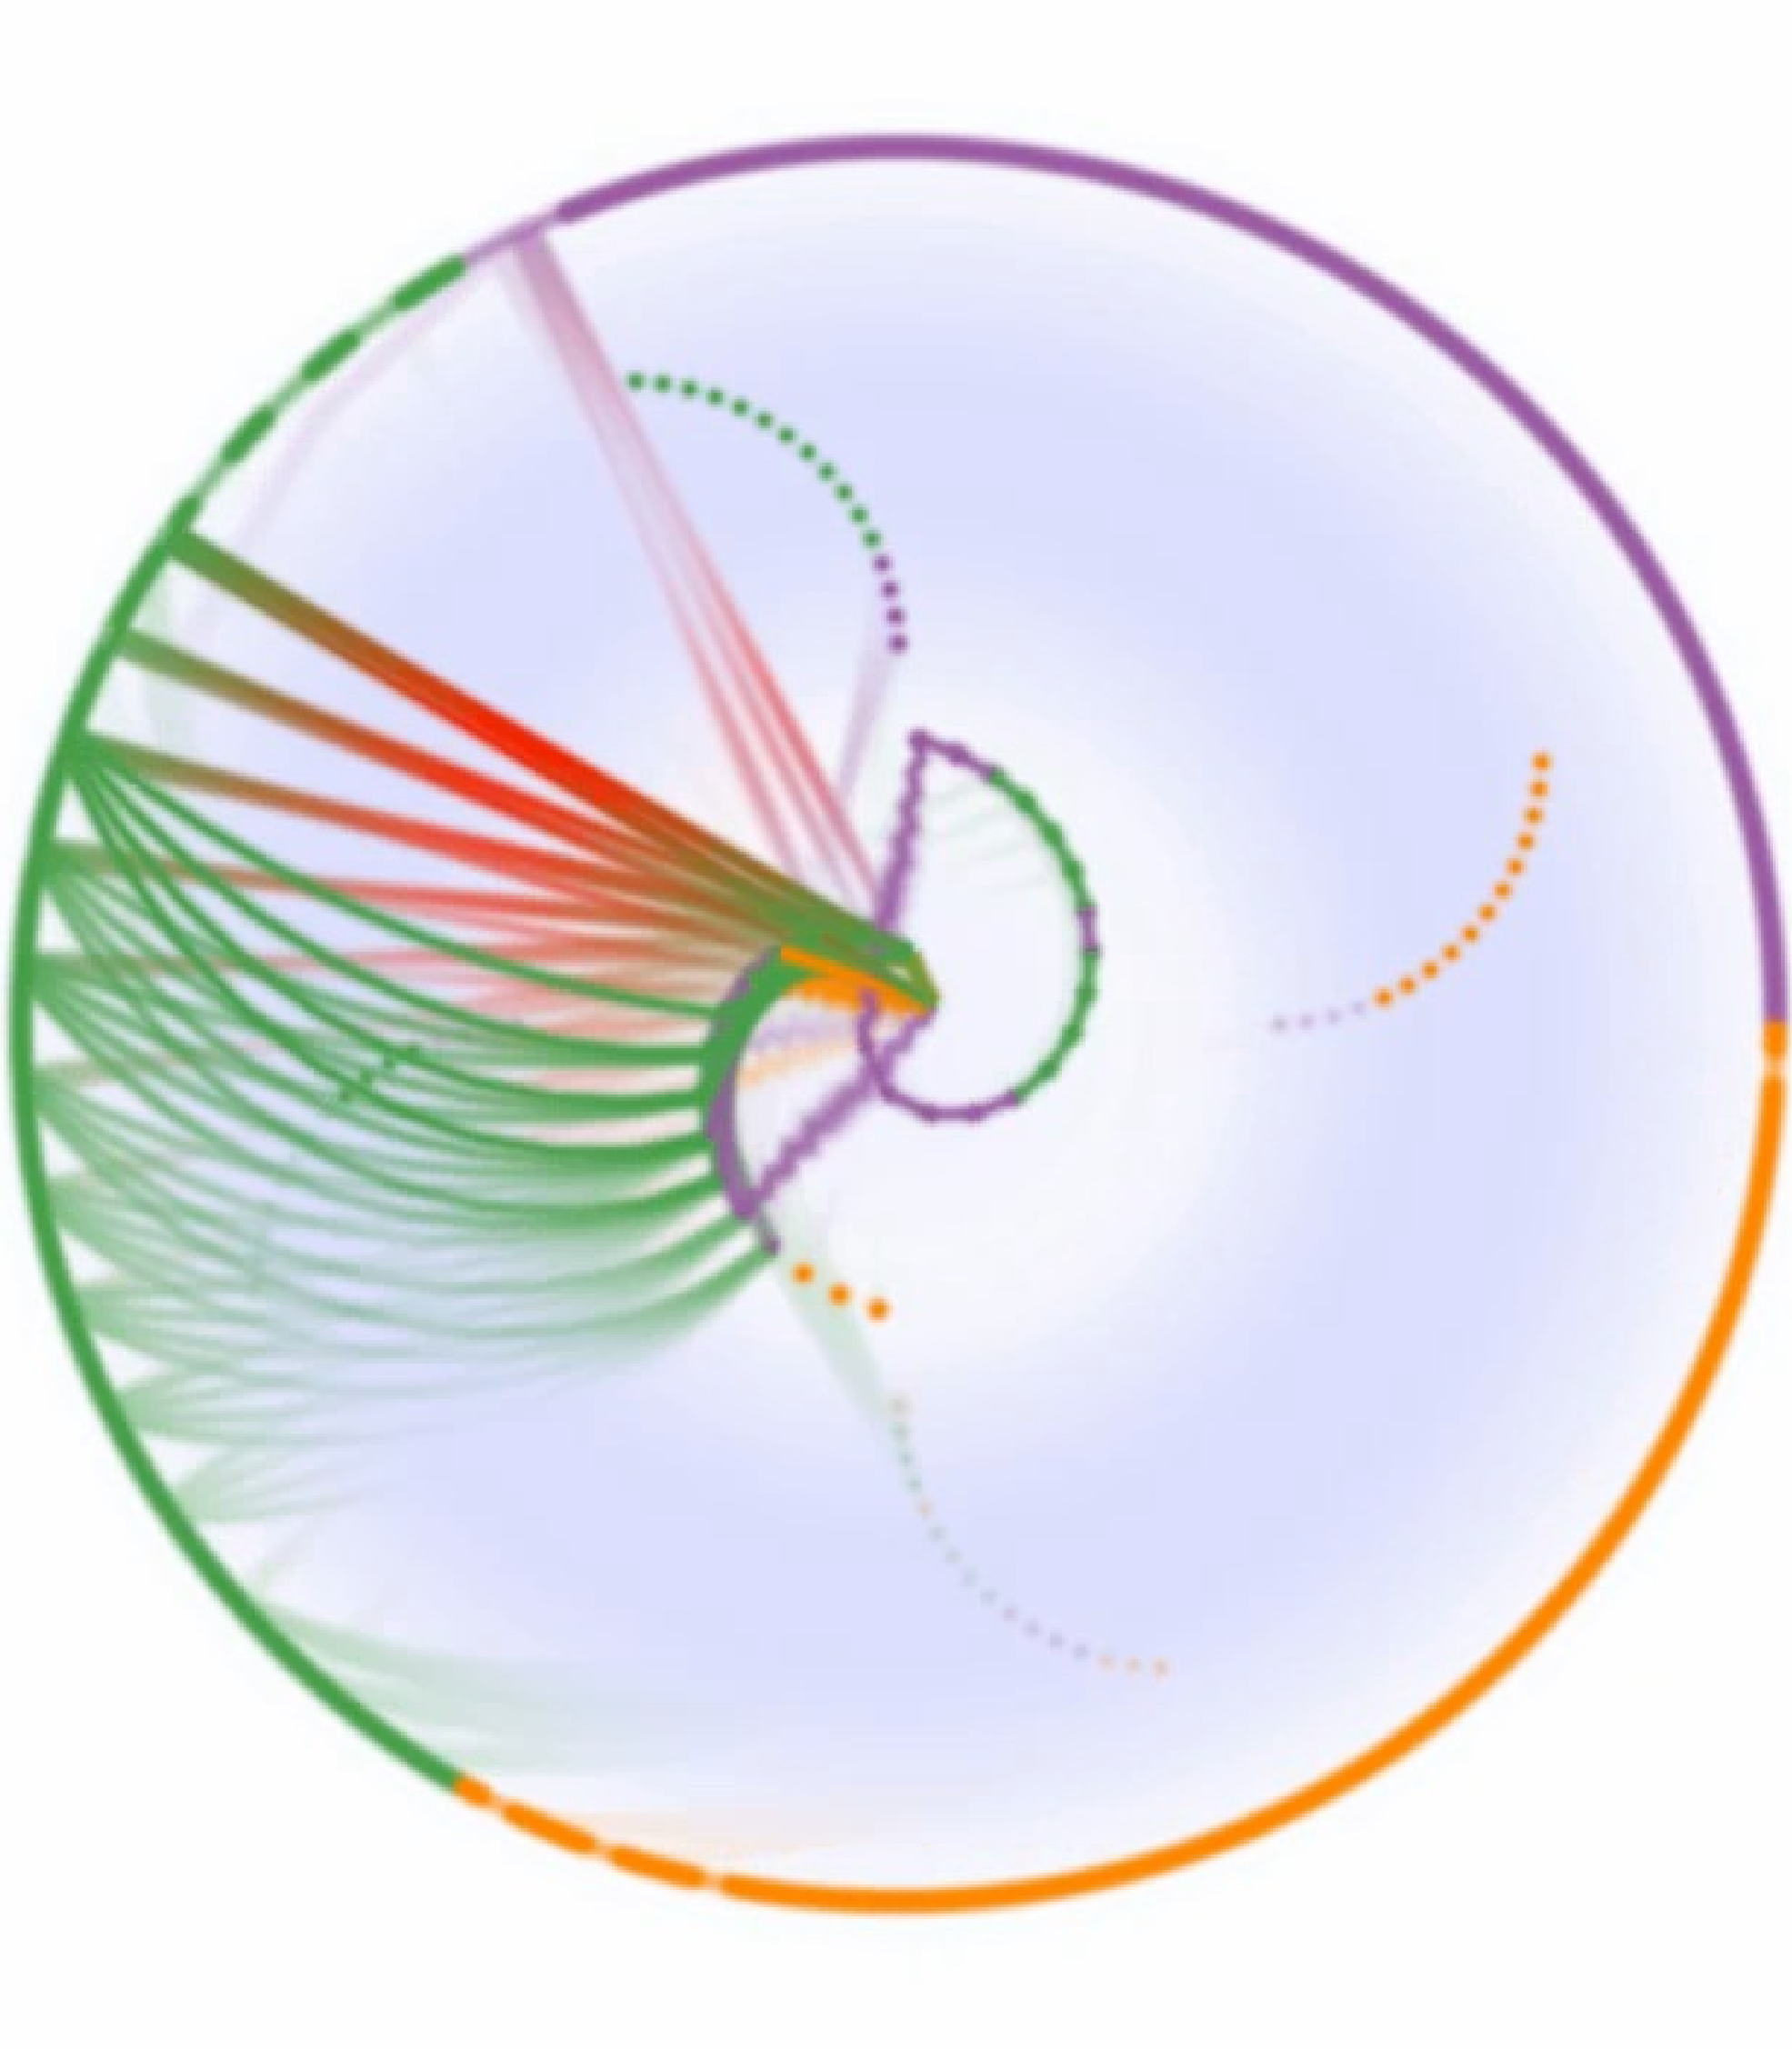
\includegraphics[width=\linewidth]{pictures/abstract_standard.png}
	\end{subfigure}
	\begin{subfigure}[c]{.24\linewidth}
		\centering
		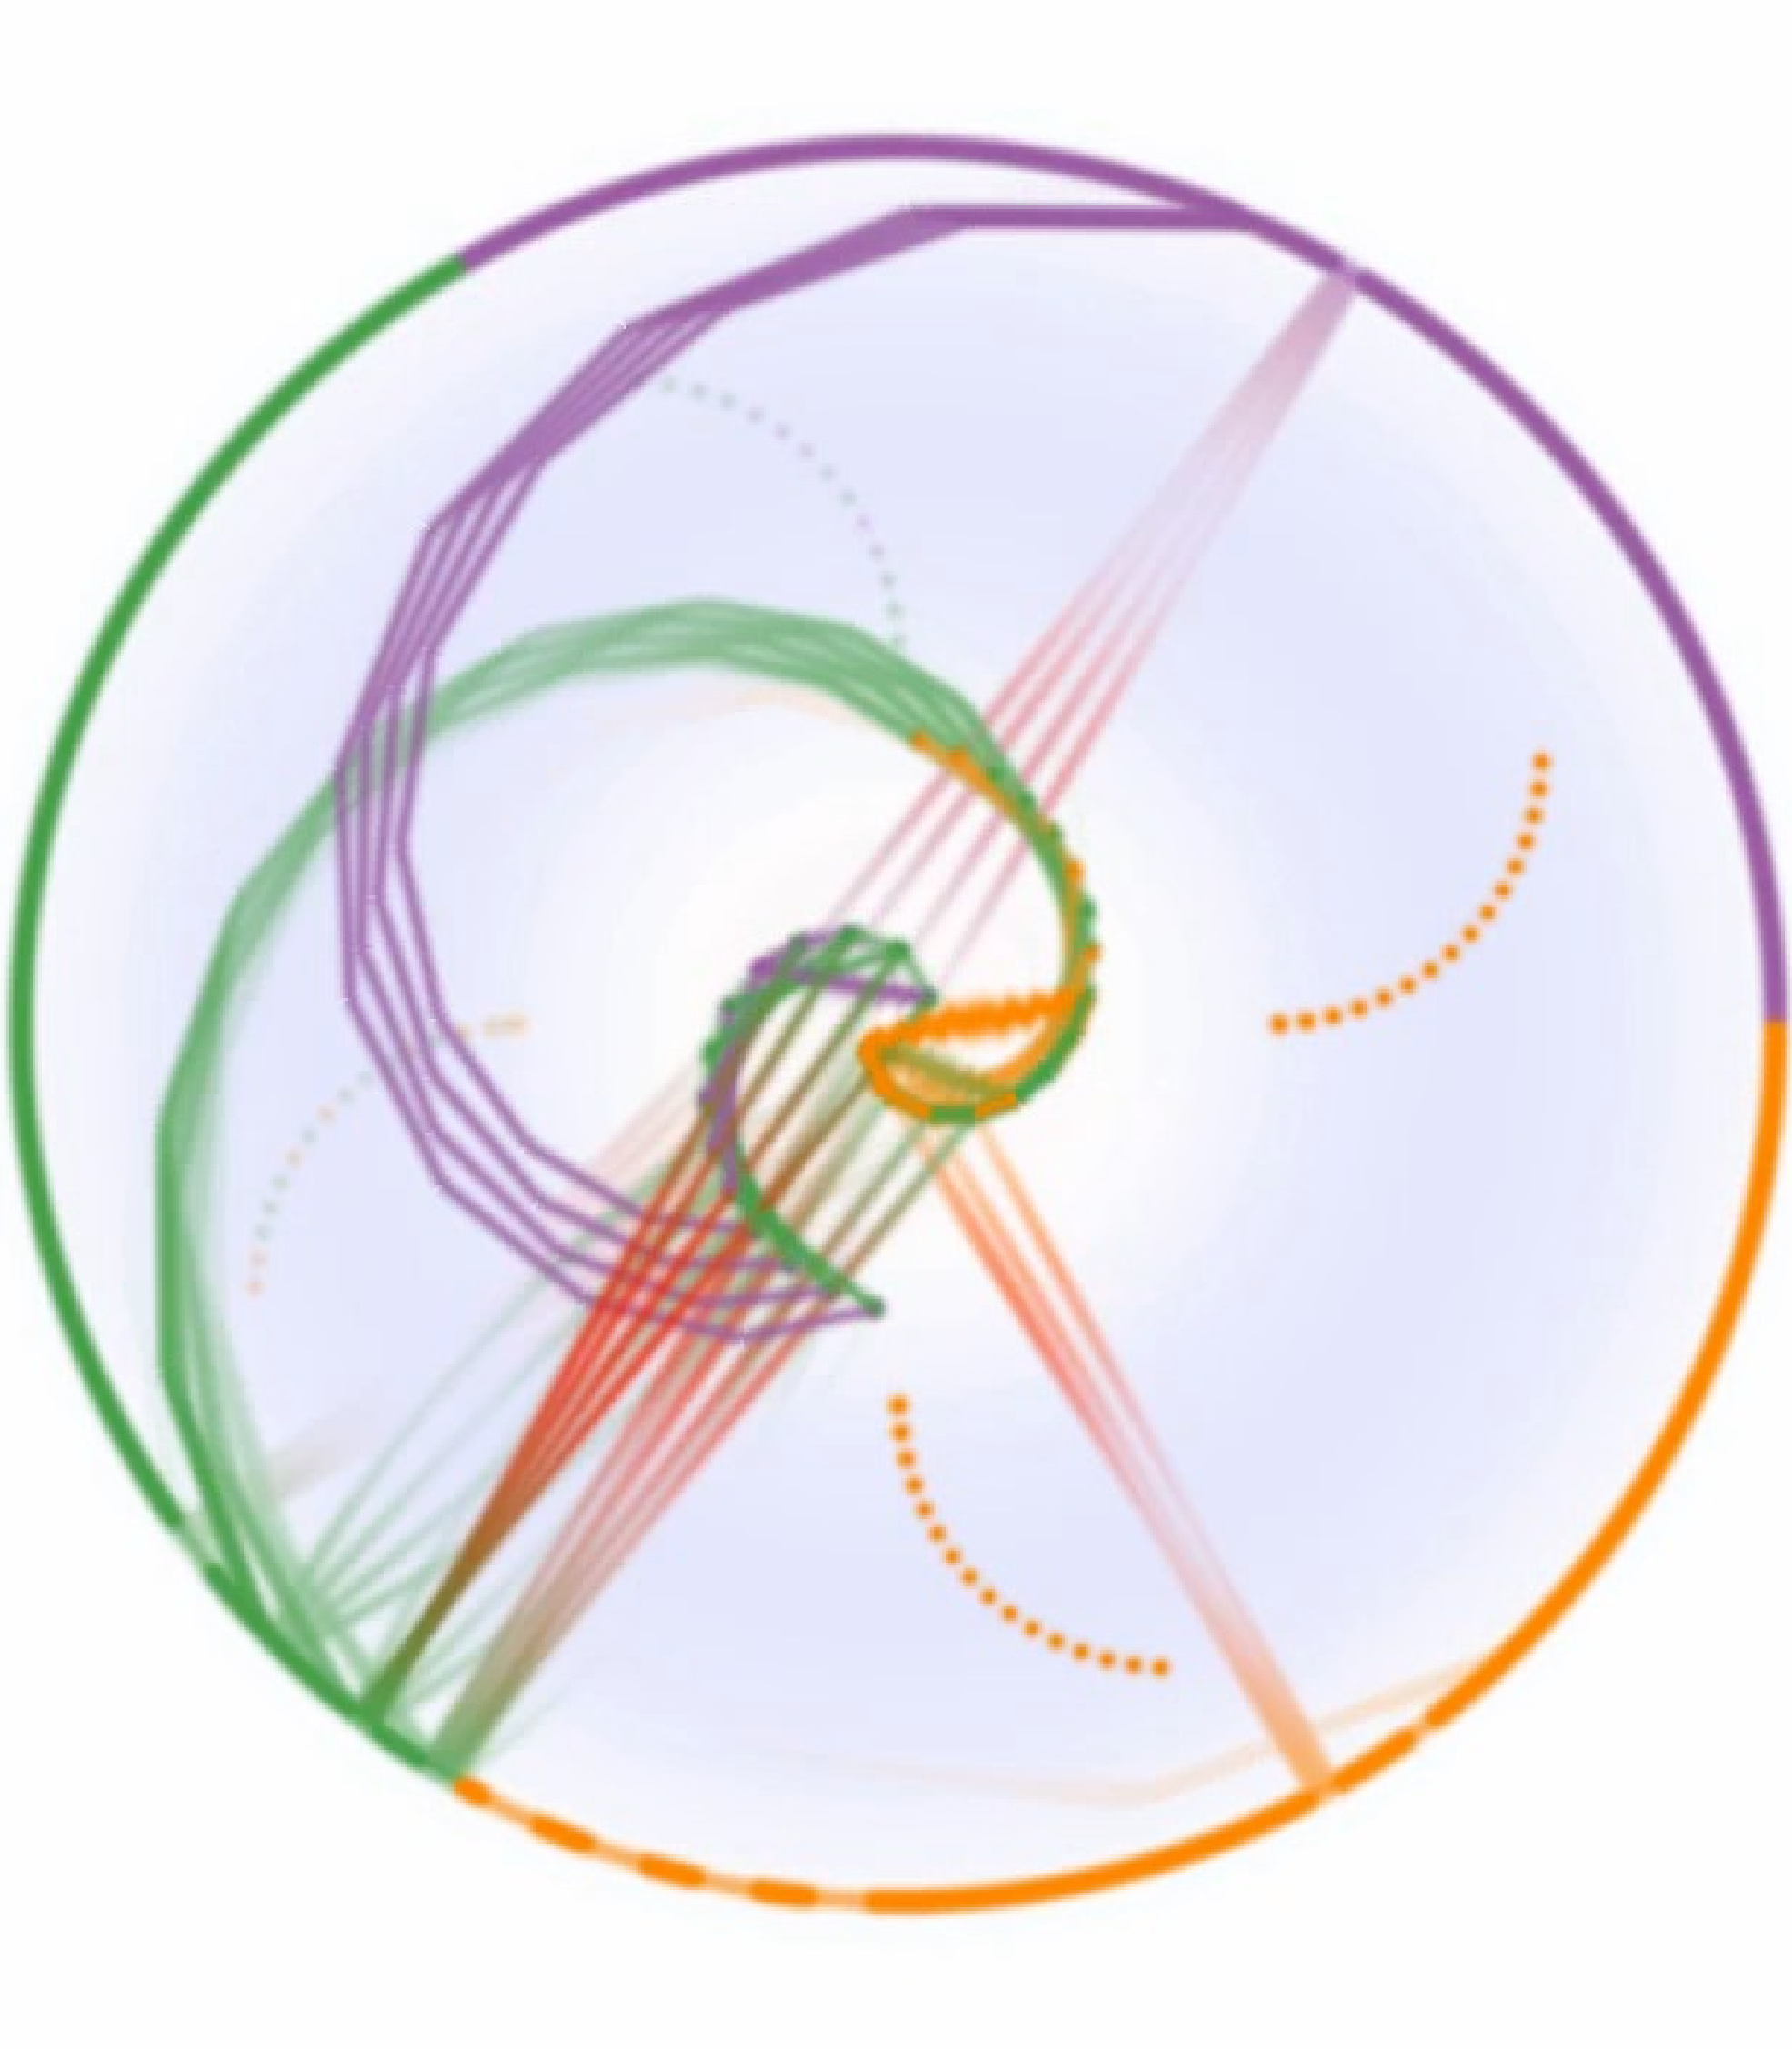
\includegraphics[width=\linewidth]{pictures/abstract_optimized.png}
	\end{subfigure}
	\caption{Left: Radial design used in \cite{choudhury2011abstract}. Glyphs arrange themselves into groupings indicating storage on the same cache, with data closer to the boundaries between the levels more likely to be evicted. Right: A comparison of a standard $16 \times 16$ matrix multiplication and an optimized version using $4 \times 4$ blocking. The standard version shows poor data reuse for two of the three matrices \cite{choudhury2011abstract}.}
	\label{fig:abstract_cache}
\end{figure*}

Visualization is an essential aspect of data locality analysis, providing the vital link between the analysis results and user comprehension. Effective visualization techniques should balance intuitiveness and informational value. Generally, visualizations for memory-related data can be classified into three categories, each catering to a specific level of detail:

\subsubsection{High-Level View}\label{sec:coarse_view}
This category of visualization provides the most abstract or "bird's eye" view of data locality, aiming to deliver a global understanding of the program's performance. It emphasizes the logical data movement behavior, spotlighting the performance impact of individual parts of the program \cite{schaad2021boosting,schaad2022boosting,gimenez2017memaxes,adhianto2010hpctoolkit}, as illustrated in Figure \ref{fig:coarse}. An integral feature of such visualizations is hierarchical clustering, which allows users to zoom into specific parts of the program, such as a loop nest. Despite providing a broad performance landscape, these visualizations do not shed light on the root causes of identified bottlenecks, warranting a more detailed examination.

\subsubsection{Intermediate-Level View}\label{sec:medium_view}
At the intermediate level, visualizations offer more detailed insights than high-level overviews, targeting specific segments of the program like functions or loops. One common technique involves displaying the hardware topology to visualize physical data movements across different levels of the memory hierarchy, as shown in Figure \ref{fig:memaxes_cache}. This more granular perspective assists in understanding performance bottlenecks and can help identify the most promising optimization opportunities \cite{gimenez2017memaxes,choudhury2011abstract}. Yet, it does not provide information about underlying problematic data layout or access patterns, necessitating a deeper, fine-grained examination.

\subsubsection{Detailed View}\label{sec:fine_view}
The detailed or fine-grained visualizations delve into specific aspects like data layout and access patterns within specific program segments, for instance, a loop nest. Figure \ref{fig:boosting_cache} displays two examples of such visualizations. The left image illustrates the data layout of a matrix, highlighting the spatial locality of elements within a cache line. The right image presents the access patterns of a loop nest, showing the correlation between accesses to different arrays. This level of visualization aids in identifying potential optimization routes, such as reshaping data to improve spatial locality or reordering the loop to enhance data access patterns \cite{schaad2022boosting}. However, these visualizations provide insights into only one program segment at a time and lack a broader picture of the program's overall data locality. Therefore, it's advisable to use a mix of visualization techniques to obtain a comprehensive understanding of a program's data locality.
